\section{逼近误差的评价}
\label{sec:dapx-error}

算法停下来以后，手里有一个候选$\widehat{Q}$和一个算出的目标值。这个近似有多好？要回答这个问题，先要把误差的来源分开，再按后续任务选择检验的量。只看一个KL数值，既分不清误差从哪里来，也不知道它对任务意味着什么。

\paragraph{三个来源}
固定一个逼近目标，记为$\mathcal{L}(Q)$，例如$D_{\mathrm{KL}}(Q\Vert\Pi)$。设族内最优解$Q^{\dagger}\in\argmin_{Q\in\mathcal{Q}}\mathcal{L}(Q)$存在，算法输出$\widehat{Q}$，报告的目标值是$\widehat{\mathcal{L}}$。三者之间有恒等式
\begin{equation}
 \widehat{\mathcal{L}}=\underbrace{\mathcal{L}(Q^{\dagger})}_{\text{表达限制}}+\underbrace{\mathcal{L}(\widehat{Q})-\mathcal{L}(Q^{\dagger})}_{\text{优化差距}}+\underbrace{\widehat{\mathcal{L}}-\mathcal{L}(\widehat{Q})}_{\text{计算误差}} .
 \label{eq:dapx-error-parts}
\end{equation}
第一项只由目标和候选集合决定，与算法无关：候选集合里最好的分布离目标也有这么远。第二项非负，衡量算法离族内最优还差多少，它可能来自迭代步数不够，也可能来自停在了局部最优。第三项来自期望的数值计算，用样本平均估计期望时它是随机的，可正可负。图~\ref{fig:dapx-error-parts}示意了前两项。

\begin{BookInlineFigure}
 \centering
 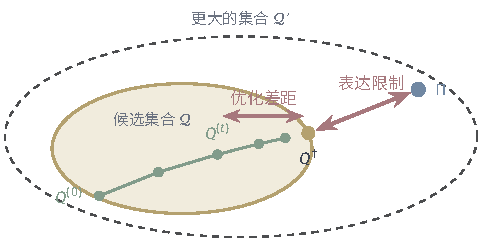
\includegraphics[width=82mm]{figures/07-probability/07-distribution-optimization/tikz/dapx-error-parts/figure.pdf}
 \caption{误差来源示意（不按比例，KL也不是几何距离）。黄色区域是候选集合$\mathcal{Q}$，蓝点是目标$\Pi$，黄点$Q^{\dagger}$是族内最优解；绿点是算法的迭代。$\Pi$到$Q^{\dagger}$的红色箭头是表达限制，迭代到$Q^{\dagger}$的红色箭头是优化差距。虚线是包含$\mathcal{Q}$的更大候选集合$\mathcal{Q}'$，它的表达限制不会更大。}
 \label{fig:dapx-error-parts}
\end{BookInlineFigure}

用四次方目标把三项都算出来。表达限制是高斯族内的最小KL，$0.0472$。第~\ref{sec:dapx-gradient}节的梯度下降做$10$步时KL为$0.0654$，优化差距是$0.0182$；做$40$步时差距已小于$10^{-4}$。计算误差来自对$J$的估计：若不用闭式~\eqref{eq:dapx-quartic-J}，而是从$Q$抽$n$个样本，用
\[
 \widehat{J}_n=\frac1n\sum_{i=1}^{n}\bigl(\ln q(X_i)-\ln\widetilde{\pi}(X_i)\bigr),\qquad X_i\sim Q\text{独立},
\]
估计$J(Q)$，它的标准差是$\sigma/\sqrt{n}$，$\sigma$是被积函数在$Q$下的标准差。在$Q^{*}$处模拟得$\sigma\approx0.409$。

$n=100$时估计的均方根误差约为$0.043$（$400$次重复，种子$727$），比第$10$步的优化差距$0.018$还大。也就是说，用$100$个样本估计目标值时，看不出第$10$步与最优解的差别；要分辨$0.018$这样的差距，需要把标准差压到它的几分之一，$n$要到几千。图~\ref{fig:dapx-mc-error}显示，误差按$n^{-1/2}$缩小，与$\sigma/\sqrt{n}$吻合。积分误差的一般理论与缩小方差的办法分别在第~\ref{chap:monte-carlo-integration-error}章和第~\ref{chap:variance-reduction}章展开。

\begin{BookInlineFigure}
 \centering
 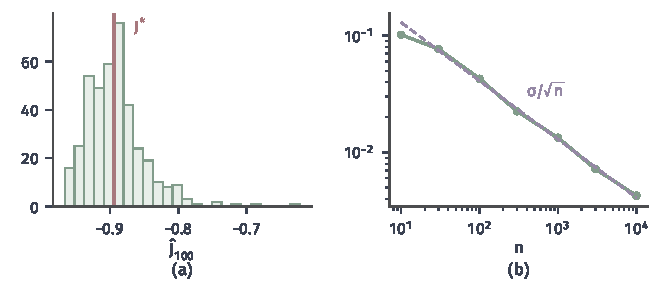
\includegraphics[width=112mm]{figures/07-probability/07-distribution-optimization/matplotlib/dapx-mc-error/figure.pdf}
 \caption{目标值的计算误差。候选为四次方目标的最优高斯$Q^{*}$，$J^{*}\approx-0.8943$。(a)$400$次独立重复中$n=100$的估计$\widehat{J}_{100}$（浅绿直方图）与真值（红线），标准差约$0.043$。(b)均方根误差随$n$的变化（绿，双对数坐标）与$\sigma/\sqrt{n}$（紫色虚线），$\sigma\approx0.409$。随机数种子为$727$。}
 \label{fig:dapx-mc-error}
\end{BookInlineFigure}

式~\eqref{eq:dapx-error-parts}还提醒一件事：当目标只有未归一化形式时，算出的是$J$而不是KL，第一项“表达限制”的大小未知，只知道$-J$是$\ln Z$的下界。比较几个候选或几个候选集合时，$J$的差就是KL的差，足以判断谁更好；要说“近似已经足够好”，则需要别的检验。

\paragraph{按任务检验}
后续任务若要用近似分布计算某些量，就应当直接检验这些量。对四次方目标，两个方向的最优高斯分别是$Q_{\mathrm{r}}=\mathcal{N}(0,0.5774)$与$Q_{\mathrm{f}}=\mathcal{N}(0,0.6760)$。比较二阶矩与四阶矩：
\[
 \begin{array}{lccc}
  & \Pi & Q_{\mathrm{r}} & Q_{\mathrm{f}}\\
 \mathbb{E}[X^{2}] & 0.676 & 0.577 & 0.676\\
 \mathbb{E}[X^{4}] & 1 & 1 & 1.371
 \end{array}
\]
目标的四阶矩由$\Gamma(5/4)=\tfrac14\Gamma(1/4)$得到：
\[
 \mathbb{E}_{\Pi}[X^{4}]=\frac{4\,\Gamma(5/4)}{\Gamma(1/4)}=1 .
\]
按目标加权的解匹配了二阶矩，这是矩匹配的直接结果，四阶矩却高估了$37\%$。按候选加权的解低估了二阶矩约$15\%$，四阶矩却恰好正确。图~\ref{fig:dapx-moment-compare}画出三个密度：目标的顶部更平、两侧下降更陡，两个高斯都无法同时匹配这两个特征。

后一个现象有原因。在候选$\mathcal{N}(0,s^{2})$中，把$X$写成$sY$，$J(s)=-\ln s-C-\mathbb{E}[\ln\widetilde{\pi}(sY)]$。对$s$求导并令其为零，再乘以$s$，得到最优尺度满足
\[
 \mathbb{E}_{Q_{\mathrm{r}}}\bigl[X\,(\ln\widetilde{\pi})'(X)\bigr]=-1 .
\]
另一方面，若$\pi$可微且$x\pi(x)\to0$（$\lvert x\rvert\to\infty$），分部积分给出
\[
 \mathbb{E}_{\Pi}\bigl[X\,(\ln\pi)'(X)\bigr]=\int x\pi'(x)\,\mathrm{d}x=-\int\pi(x)\,\mathrm{d}x=-1 .
\]
两式的左边是同一个函数$x(\ln\widetilde{\pi})'(x)$在两个分布下的期望。四次方目标中这个函数是$-x^{4}$，所以两个分布的四阶矩相同。可见，每个方向只“保留”与自己的驻点方程相关的那些平均，其余的量要单独检验。

\begin{BookInlineFigure}
 \centering
 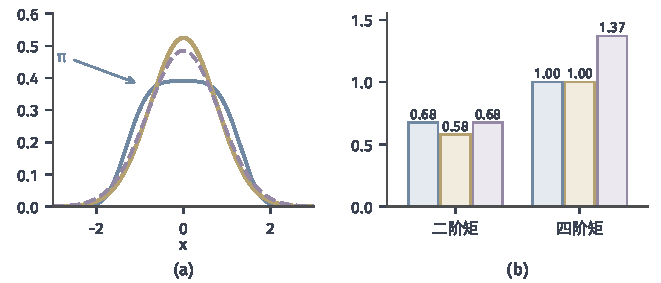
\includegraphics[width=112mm]{figures/07-probability/07-distribution-optimization/matplotlib/dapx-moment-compare/figure.pdf}
 \caption{四次方目标的两个高斯近似。(a)目标密度（蓝），按候选加权的最优解$\mathcal{N}(0,0.577)$（黄），按目标加权的最优解$\mathcal{N}(0,0.676)$（紫色虚线）。(b)三个分布的二阶矩与四阶矩，颜色同(a)。}
 \label{fig:dapx-moment-compare}
\end{BookInlineFigure}

关心事件概率时，可以用第~\ref{chap:distribution-comparison}章的Pinsker不等式$d_{\mathrm{TV}}\leq\sqrt{D_{\mathrm{KL}}/2}$。总变差是对称的，两个方向的KL都可以代入。对$Q_{\mathrm{r}}$，$D_{\mathrm{KL}}(Q_{\mathrm{r}}\Vert\Pi)\approx0.0472$给出$d_{\mathrm{TV}}\leq0.154$，数值积分得到的真值是$0.115$。对$Q_{\mathrm{f}}$，$D_{\mathrm{KL}}(\Pi\Vert Q_{\mathrm{f}})\approx0.0317$给出$d_{\mathrm{TV}}\leq0.126$，真值是$0.094$。这个上界对所有事件同时成立，但对具体的事件往往很松：$\mathbb{P}(\lvert X\rvert>1.5)$在目标下是$0.0462$，在$Q_{\mathrm{r}}$下是$0.0484$，在$Q_{\mathrm{f}}$下是$0.0681$，按候选加权的近似在这个尾概率上反而更好。

\paragraph{无界的检验函数}
若要检验的是无界函数的期望，比如矩，总变差和KL本身都不够，必须有尾部条件。第~\ref{chap:distribution-comparison}章证明了：KL要控制$g$的期望差，需要$g$在参考分布下有指数矩。反例很简单。目标为标准Cauchy分布、候选为高斯分布时，第~\ref{sec:dapx-target-candidates}节已经看到$D_{\mathrm{KL}}(Q\Vert\Pi)$有限，可是$\mathbb{E}_{\Pi}[X^{2}]=+\infty$，而每个高斯候选的二阶矩都有限。无论KL被优化到多小，用这个近似计算二阶矩都没有意义。所以，按任务检验时要先确认待求的量在目标下存在，再确认所用的比较量能控制它。

\paragraph{扩大候选集合}
若$\mathcal{Q}\subset\mathcal{Q}'$，则
\[
 \inf_{Q\in\mathcal{Q}'}\mathcal{L}(Q)\leq\inf_{Q\in\mathcal{Q}}\mathcal{L}(Q) ,
\]
因为在更大的集合里取下确界，可选的更多。这只说明式~\eqref{eq:dapx-error-parts}的第一项不会变大，并不说明实际算出的结果会变好：更大的候选集合往往带来更难的优化，第二项可能变大。

看式~\eqref{eq:dapx-bimodal}的双峰目标，目标值取$D_{\mathrm{KL}}(Q\Vert\Pi)$。单个高斯族内的最小值约为$0.356$，在左峰。两成分高斯混合族（权重、均值、方差都可变）包含目标本身，下确界为$0$。设对混合族做梯度下降，两个成分的权重都初始化为$\tfrac12$，均值和方差也取相同的值，放在右峰附近。交换两个成分不改变混合分布，所以目标值关于两组成分参数对称；在两组参数相同的点上，目标值对两组参数的偏导数也相同，每一步更新都保持两个成分相同，权重也一直是$\tfrac12$。这样的混合就是单个高斯，迭代实际上是在单个高斯族里进行，会停在右峰的局部最小点，值约为$1.202$。图~\ref{fig:dapx-larger-family}对比了这几个数。

\begin{BookInlineFigure}
 \centering
 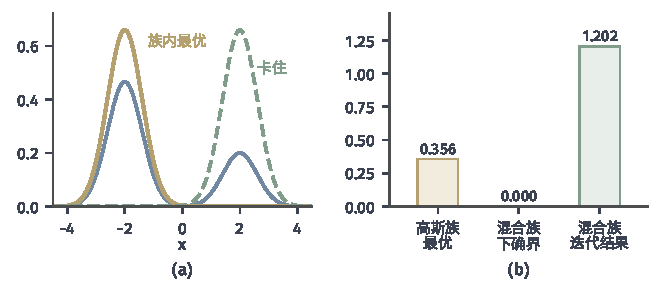
\includegraphics[width=112mm]{figures/07-probability/07-distribution-optimization/matplotlib/dapx-larger-family/figure.pdf}
 \caption{扩大候选集合不保证结果变好。(a)双峰目标（蓝）、单个高斯族内按候选加权的最优解$\mathcal{N}(-2,0.6^{2})$（黄），以及两成分完全相同地初始化在右峰附近的混合族迭代的结果（绿色虚线），它停在右峰的单个高斯上。(b)$D_{\mathrm{KL}}(Q\Vert\Pi)$：高斯族最优$0.356$，混合族下确界$0$，混合族迭代结果$1.202$。}
 \label{fig:dapx-larger-family}
\end{BookInlineFigure}

这个例子是刻意构造的，但它揭示的机制普遍存在：候选集合越大，目标函数的局部最优和对称结构往往越多。比较两个候选集合时，应当比较实际算出的结果，并报告初值与迭代设置；“族更大所以更准”只对下确界成立。
